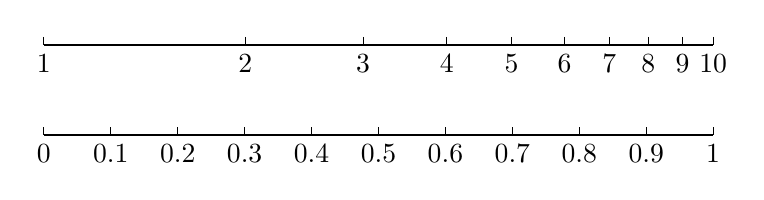
\begin{tikzpicture}[declare function={logdist(\x)=\xscale*log10(\x);}]%
  \node at (0, 0) {};
  \pgfmathsetmacro{\xscale}{8.5}
  \pgfmathsetmacro{\y}{-1.25}
  \draw[thick] (0,\y) -- (\xscale,\y);
  \foreach \x in {0.,0.1,...,1.1}
  \draw (\x*\xscale,\y+0.1) -- (\x*\xscale,\y) node[anchor=north]
        {$\pgfmathprintnumber{\x}$};
        
  \pgfmathsetmacro{\y}{-0.1}
  \draw[thick] (0,\y) -- (\xscale,\y);
  \foreach \x in {1,...,10}
  \draw ({logdist(\x)},\y+0.1) -- ({logdist(\x)},\y) node[anchor=north]
        {$\pgfmathprintnumber{\x}$};
\end{tikzpicture}
